\documentclass[12pt,titlepage]{report}
\usepackage[utf8]{inputenc}
\usepackage[slovene]{babel}
\usepackage{graphicx}
\usepackage{setspace}
\usepackage{mathptmx}
\usepackage{pdfpages}
\usepackage{setspace}
\usepackage{csquotes}
\usepackage{float}
\usepackage{multicol}
\usepackage{amssymb,amsmath,mathtools,mathrsfs}
\usepackage[T1]{fontenc}% http://ctan.org/pkg/fontenc
\usepackage{tikz}
\usepackage{titlesec}
\usepackage{titletoc}
\usepackage{subcaption}
\usepackage{listings}
\usepackage[backend=biber, maxbibnames=99, sorting=none]{biblatex}
\addbibresource{bibliography.bib}
\usepackage{vegovatitle}
\usepackage[
        a4paper,% other options: a3paper, a5paper, etc
        left=3cm,
        right=2.5cm,
        top=2.5cm,
        bottom=2.5cm,
        % use vmargin=2cm to make vertical margins equal to 2cm.
        % us  hmargin=3cm to make horizontal margins equal to 3cm.
        % use margin=3cm to make all margins  equal to 3cm.
]{geometry}

\setlength{\parskip}{1em}
\DeclareQuoteAlias{croatian}{slovene}
%\renewcommand\thesection{\arabic{section}}
\linespread{1.5}
\setlength{\parindent}{0pt}

% Format poglavij
\titleclass{\chapter}{straight}
\titleformat{\chapter}[hang]
{\normalfont\LARGE\bfseries}
{\LARGE\thechapter.}
{0.5em}
{}
\titlespacing{\chapter}{0pt}{10pt}{10pt}

\title{KALKULATOR}
\project{Strokovno poročilo}
\author{Rok Strah, R 4. C}
\mentor{Darjan Toth, prof.}

\lstset{%
	frameround=single,%
	xleftmargin = \parindent%
}

\newcommand{\wdot}{\textcolor{white}{.}}
\newcommand{\odstavek}{\wdot \\ \wdot \qquad}
\newcommand{\codequote}[1]{\textquote{\texttt{#1}}}
\newcommand{\angokr}[2]{(okrajšano #1 iz angl. \emph{#2})}
\newcommand{\group}[2]{\parbox{#1}{\setstretch{0.5}\vspace{5pt}\texttt{#2}\vspace{5pt}}}
\newenvironment{alignitemize}
{

\begin{tabular}{@{$\bullet$ }ll}
}{
\end{tabular}

}

\begin{document}

\maketitle

\chapter*{Povzetek}
\chapter*{Abstract}
\thispagestyle{empty}


{\begin{spacing}{1.15}
\pagestyle{empty}
\clearpage
\tableofcontents
\clearpage
\listoffigures
\pagestyle{plain}
\end{spacing}}
\thispagestyle{empty}
\clearpage
\setcounter{page}{1}

\chapter{Uvod}
\label{intro}

\chapter{Metodologija}
\label{methods}
	\section{Okolje, orodja, jezik in standardi}
		Za projekt sem uporabil programski jezik C++, razvojno orodje Qt Creator in nekaj knjižnic.
		\subsection{C++}			
			C++ je Bjarne Stroustrup kot razširitev C-ju naredil v letu 1979.
			Želel je ustvariti učinkovit in prilagodljiv jezik podoben C-ju, ki pa bi tudi imel visoko-nivojske funkcije za organizacijo programa, kot so razredi.
			C++ je ISO/IEC JTC 1/SC 22/WG 21 standardizirala leta 1998, in od takrat so izdali 5 standardov:\cite{cpp_wiki}
			\begin{itemize}
				\item ISO/IEC 14882:1998 znan kot C++98,
				\item ISO/IEC 14882:2003 znan kot C++03,
				\item ISO/IEC 14882:2011 znan kot C++11 ali C++0x,
				\item ISO/IEC 14882:2014 znan kot C++14 ali C++1y in
				\item ISO/IEC 14882:2017 znan kot C++17 ali C++1z,
			\end{itemize}
			sedaj pa delajo na naslednjem standardu, ki naj bi prišel v letu 2020 in je znan pod imenom C++20.
			\odstavek
			Bjarne je leta 1979 začel razvijati \textquote{C with Classes}, razširitev C-ju in predhodnik C++.
			Ko je delal na doktorski nalogi, je opazil, da ima jezik \textquote{Simula} nekaj funkcij, ki so zelo uporabne za velike projekte, vendar je prepočasen za praktično rabo, vendar pa jeziku \textquote{BCPL}, ki je hiter, manjkajo visoko-nivojske funkcije za večje projekte.
			Med delom v \textquote{AT\&T Bell Labs} je bil navdihnjen izboljšati C s funkcijami podobnimi tistim v Simuli.
			Izbral si je C, ker je fleksibilen, učinkovit, dostopen in prenosljiv.
			Poleg vplivov C in Simule, so na C++ vplivali tudi drugi jeziki, kot so ALGOL 68, Ada, CLU in ML.
			Leta 1983 se je \textquote{C with Classes} preimenoval v C++, leta 1989 je pa bil dokončan C++ 2.0.
			\odstavek Bjarne je medtem tudi pisal knjigo \textquote{The C++ Programming Language}.
			Do sedaj je knjiga izšla v štirih izvodih v letih: \cite{the_cpp_programming_language_wiki}
			\begin{itemize}
				\item 1985,
				\item 1991,
				\item 1997 in
				\item 2013
			\end{itemize}
			ter v eni posebni izdaji leta 2000.
			Po C++ 2.0 se je C++ razvijal relativno počasi do 2011, ko je izšel standard C++11, ki je dodal veliko novih funkcij in je razširil \textquote{standard library} (okrajšano STL).
			Trenutno je C++, za Javo in C-jem, tretji najbolj znan programski jezik.~\cite{tiobe}
			\subsubsection{Filozofija C++ \cite{cpp_wiki,cpp_evolution}}
				\begin{itemize}
					\item Splošna pravila:
					\begin{itemize}
						\item Evolucija c++ morejo voditi resnični problemi.
						\item Ne ukvarjaj se z nesmiselnim iskanjem popolnosti.
						\item C++ more biti uporaben zdaj.
						\item Vsaka funkcija jezika mora imeti razumno očitno implementacijo.
						\item Vedno zagotovi prehodno pot.
						\item C++ je jezik, ne popoln sistem.
						\item Zagotovi celovito podporo za vsak podprt slog.
						\item Ne poskušaj siliti ljudi, naj uporabljajo specifičen programski slog.
					\end{itemize}
					\item Pravila za podporo oblike:
					\begin{itemize}
						\item Podpiraj smiselne oblikovne ideje.
						\item Zagotovi metode za organizacijo programa.
						\item Reči kar misliš.
						\item Vse funkcije morejo biti cenovno dostopne.
						\item Bolj je pomembno dovoliti uporabno funkcijo, kot pa preprečiti vsako zlorabo.
						\item Podpiraj sestavljanje programske opreme iz ločeno razvitih delov.
					\end{itemize}
					\item Jezikovno-tehnična pravila:
					\begin{itemize}
						\item Nobenih implicitnih kršenj statičnega sistema tipov.
						\item Zagotovi tako dobro podporo za uporabniško-definirane tipe kot za vgrajene tipe.
						%\item \textquote{Locality} je dober.
						\item Izogibaj se zaporednih odvisnosti.
						\item Če si v dvomu, izberi varianto funkcije, ki jo je najlažje naučiti. % katero?
						\item Sintaksa je važna (ponavadi na čudne načine)
						\item Uporaba predprocesorja naj bi bila odpravljena.
					\end{itemize}
					\item Pravila za podporo nizko-nivojskega programiranja:
					\begin{itemize}
						\item Uporabljaj tradicionalne (neumne) povezovalnike (angl. \textquote{linker}).
						\item Nobenih neupravičenih nezdružljivosti s C.
						\item Ne pusti mesta za nizko-nivojski jezik pod C++ razen ASM.
						\item Za kar ne uporabljaš, ne plačaš (angl. zero-overhead rule).
						\item Če si v dvomu, zagotovi možnost za ročni nadzor.
					\end{itemize}
				\end{itemize}
		\subsection{Qt}
			Qt ([kjut] angl. \textquote{\emph{cute}}\cite{qt_pron}) je odprtokodno ogrodje za C++, ki ponuja razvojno okolje \textquote{Qt~Creator} \angokr{IDE}{Integrated~Development~Enviroment}, oblikovalec vmesnikov \textquote{Qt~Designer}, prevajalec \textquote{Qt~Linguist} in \textquote{Qt~Assistant}, ki kaže dokumentacijo in primere uporabe Qt knjižnic.
			V \textquote{Qt~Creator} imajo uporabniki na voljo tudi dostop do drugih treh programov.
			Qt knjižnice ločimo od drugih po njihovi predponi \textquote{\emph{Q}}--.
			Qt ima veliko funkcij, vendar najpomembnejše so pred-procesor moc~(iz~angl.~Meta-Object~Compiler\cite{qt_moc}), Qt knjižnica gradnikov (Qt Widgets) in Qt signali in reže (Signals \& Slots), s katerimi lahko nadziramo grafični vmesnik \angokr{GUI}{Graphical~User~Interface}.
			\subsubsection{Signali\cite{qt_signals}}
				Qt uporabnikom zagotavlja funkcije, za povezovanje signalov na reže. To sta \codequote{connect} in \codequote{disconnect}.
				Signali se ponavadi sprožijo, ko se objekt (angl.~object) spremeni, pa bi to želeli sporočiti njegovemu staršu (angl.~parent).
				Ko si signal sproži se ponavadi reže povezane nanj takoj izvedejo, kot navaden klic funkcije, \cite{qt_signals}
				vendar pa če uporabljamo zaporedne povezave (angl.~queued~connections) koda normalno nadaljuje z izvajanjem in se reže začnejo izvajati šele kasneje. \cite{qt_signals}
			\subsubsection{Reže\cite{qt_slots}}
				Reže so navadne funkcije, na katere pa lahko povežemo signale.
		\subsection{Knjižnice}
			\subsubsection{Exprtk\cite{exprtk,exprtk_git}}
				Exprtk je knjižnica za računanje za C++.
			\subsubsection{KLFBackend\cite{qt_klf}}
				KLFBackend je C++ knjižnica za prikazovanje \LaTeX{} kode.
			\subsubsection{MufExprtkBackend}
				MufExprtkBackend je vmesnik med Qt programom in knjižnico Exprtk.
				Ker se ta knjižnica ne spreminja pogosto, jo lahko prevedemo posebej od aplikacije, kar skrajša čas prevajanja aplikacije za 1 do 10 minut, odvisno od zmogljivosti procesorja.
			\subsubsection{MufTranslate}
				MufTranslate je knjižnica, ki sem jo uporabil za prevajanje vmesnika v različne jezike.
				Za razliko od Qt Linguist knjižnica podpira prevode v obliki JSON datoteke.
		
		\subsection{Linux}
			Linux je družina prostih in odprto-kodnih operacijskih sistemov, ki za jedro (angl. \emph{kernel}) uporabljajo \textquote{Linux}.
			Aplikacijo sem začel razvijati na Windows operacijskem sistemu, vendar sem moral zaradi omejitev sistema zamenjati na Linux. %TODO: expand?
			
		\subsection{Druga orodja in standardi}
			\subsubsection{AStyle\cite{astyle}}
				AStyle je program, ki samodejno oblikuje izvorno kodo po definiciji, ki jo podaš.
				Qt tudi omogoča povezavo preko dodatkov (angl. plugin);
			\subsubsection{CMake\cite{cmake}}
				CMake je prosta in odprto-kodna rešitev za avtomatizacijo grajenja projektov.
				V primerjavi s Qt-ovim qmake je močnejši, vendar zahtevnejši za uporabo.
			\subsubsection{Ninja\cite{ninja}}
				Ninja je prost odprto-kodni sistem za grajenje projektov.
				Za razliko od ostalih takih sistemov je bistveno hitrejši.
				Sicer ga je možno uporabljati samega, je mišljeno, da se ga uporablja v povezavi z programom, ki generira \codequote{.ninja} datoteke, kot je CMake.
			\subsubsection{Clang\cite{clang}}
				Clang je prost odprto-kodni vmesnik za jezike družine C, ki se od GCC-ja razlikuje predvsem po boljših sporočilih in hitrosti.
			\subsubsection{JSON\cite{json}}
				JSON (iz angl. \emph{JavaScript Object Notation}) je način zapisa tabel in objektov v tekstovno datoteko.
				Struktura JSON:\cite{json}
				\begin{itemize}
					\item JSON dokument je sestavljen iz objekta ali tabele.
					\item JSON objekt je sestavljen iz parov ključev in vrednosti. \ref{fig:json_obj}.
					\item JSON tabela vsebuje več vrednosti.\ref{fig:json_arr}
					\item Ključ je niz, vrednost je pa lahko niz, število, tabela, objekt, dvojiška vrednost (true in false) ali null.\ref{fig:json_val} \ref{fig:json_str} \ref{fig:json_num}
				\end{itemize}
			\begin{figure}[H]
				\centering
				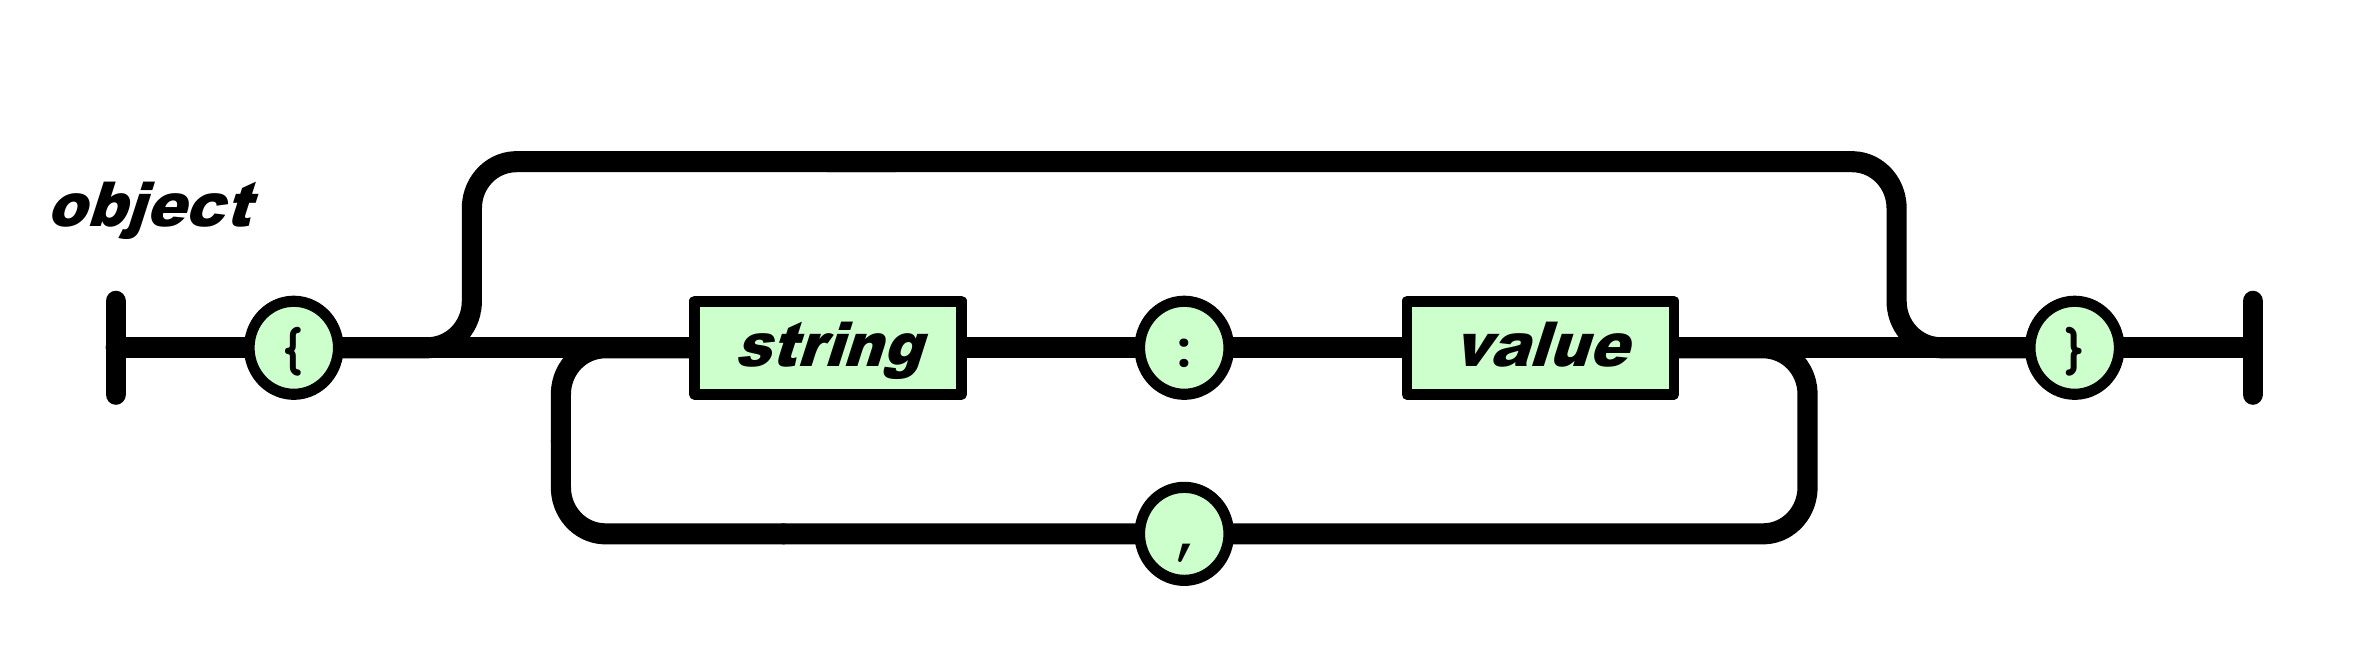
\includegraphics[width=\textwidth]{json_object.png}
				\caption{JSON objekt\cite{ecma404}}
				\label{fig:json_obj}
			\end{figure}
			\begin{figure}[H]
				\centering
				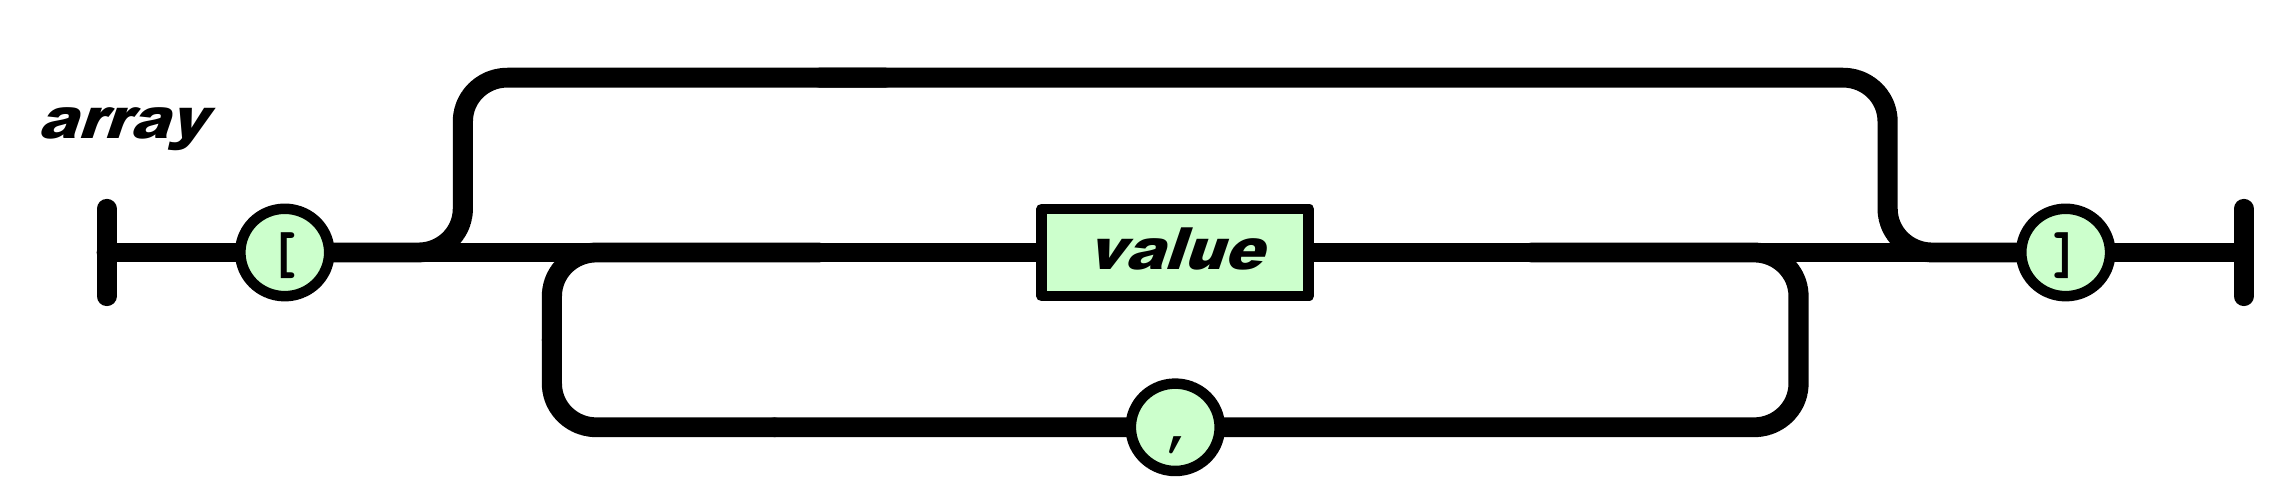
\includegraphics[width=\textwidth]{json_array.png}
				\caption{JSON tabela\cite{ecma404}}
				\label{fig:json_arr}
			\end{figure}
			\begin{figure}[H]
				\centering
				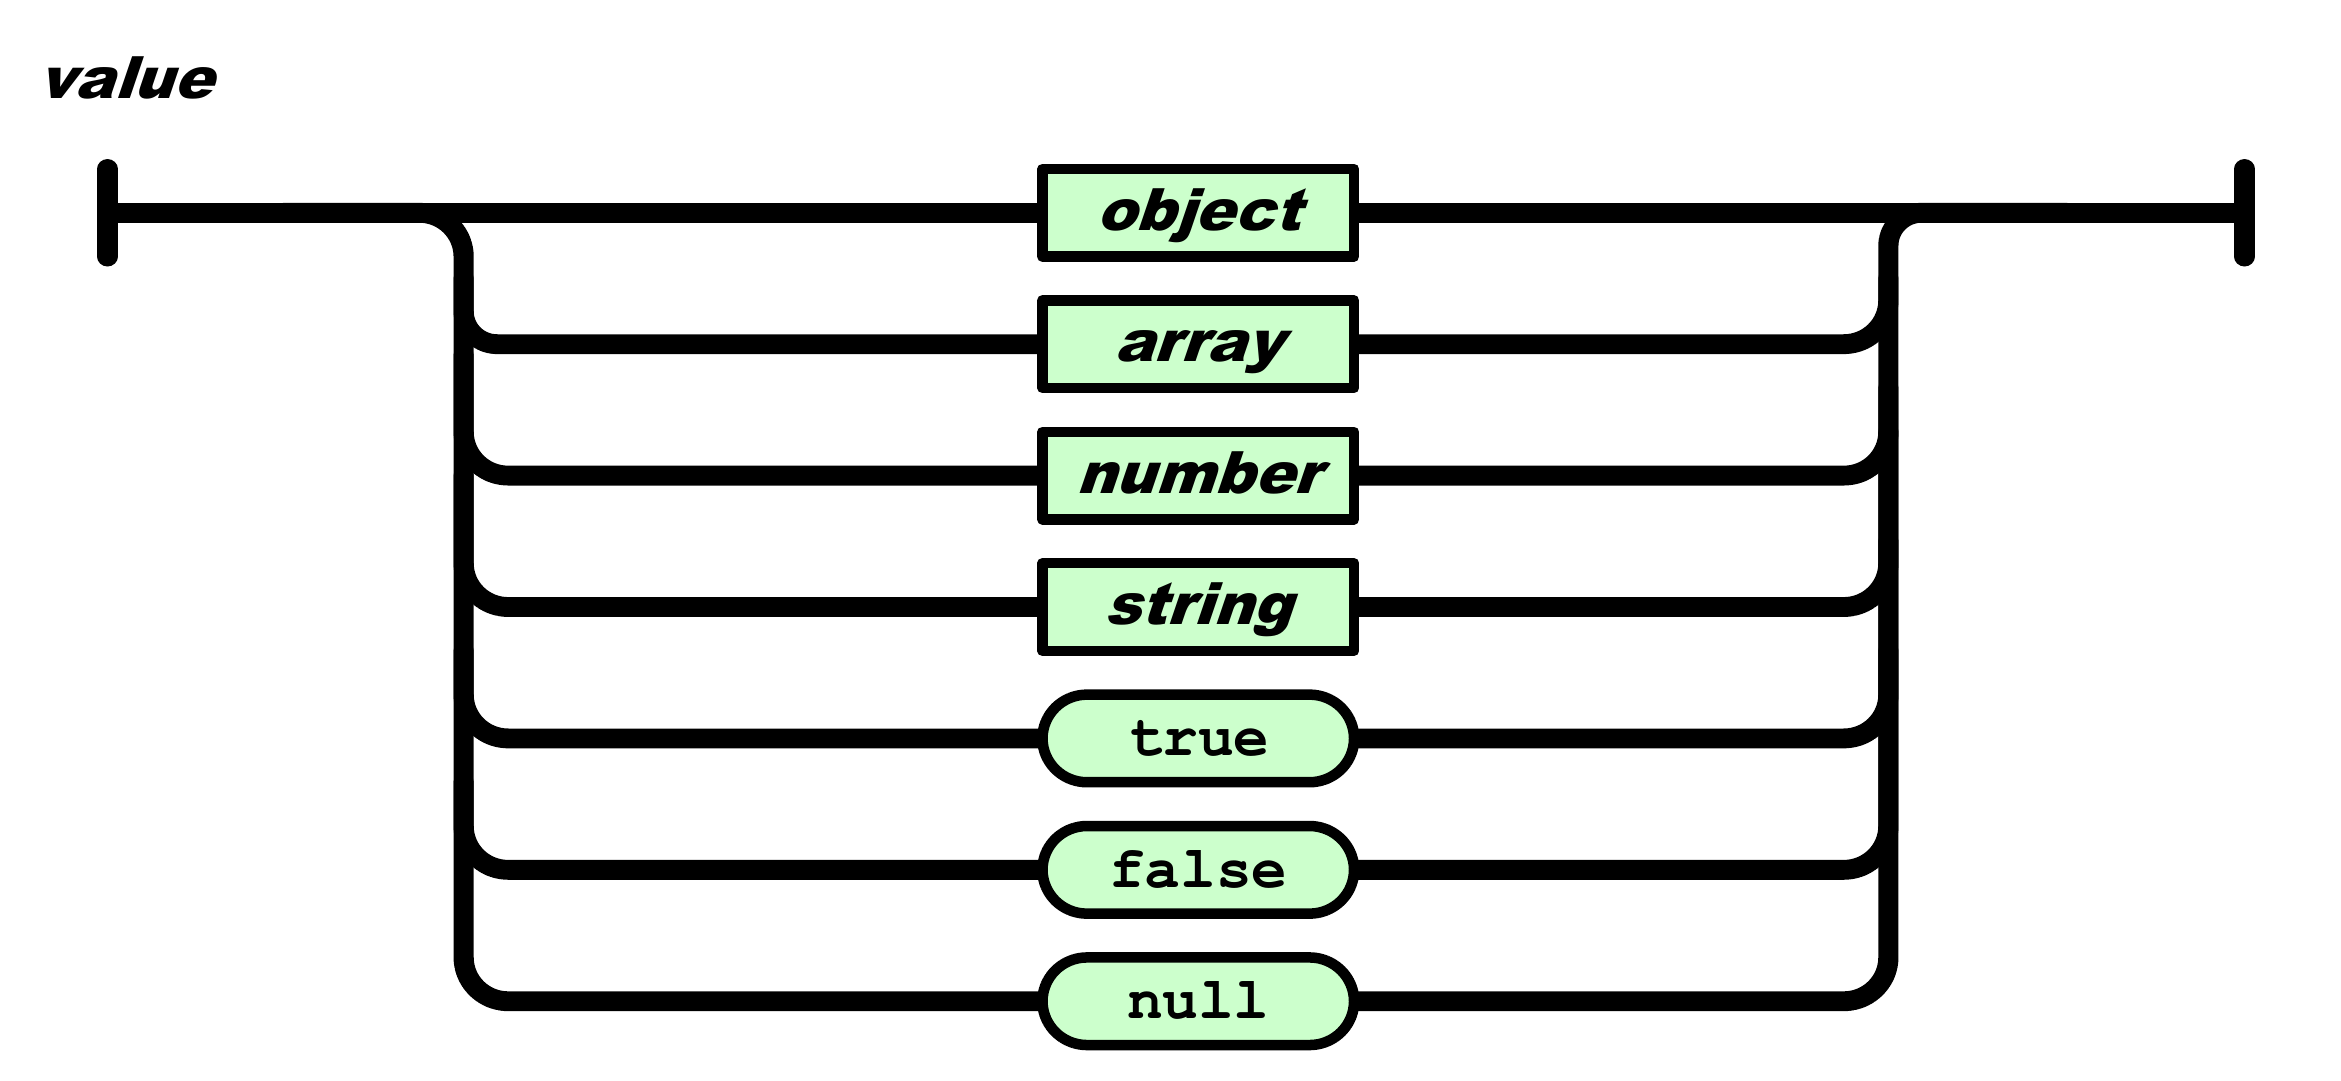
\includegraphics[width=\textwidth]{json_value.png}
				\caption{JSON vrednost\cite{ecma404}}
				\label{fig:json_val}
			\end{figure}
			\begin{figure}[H]
				\centering
				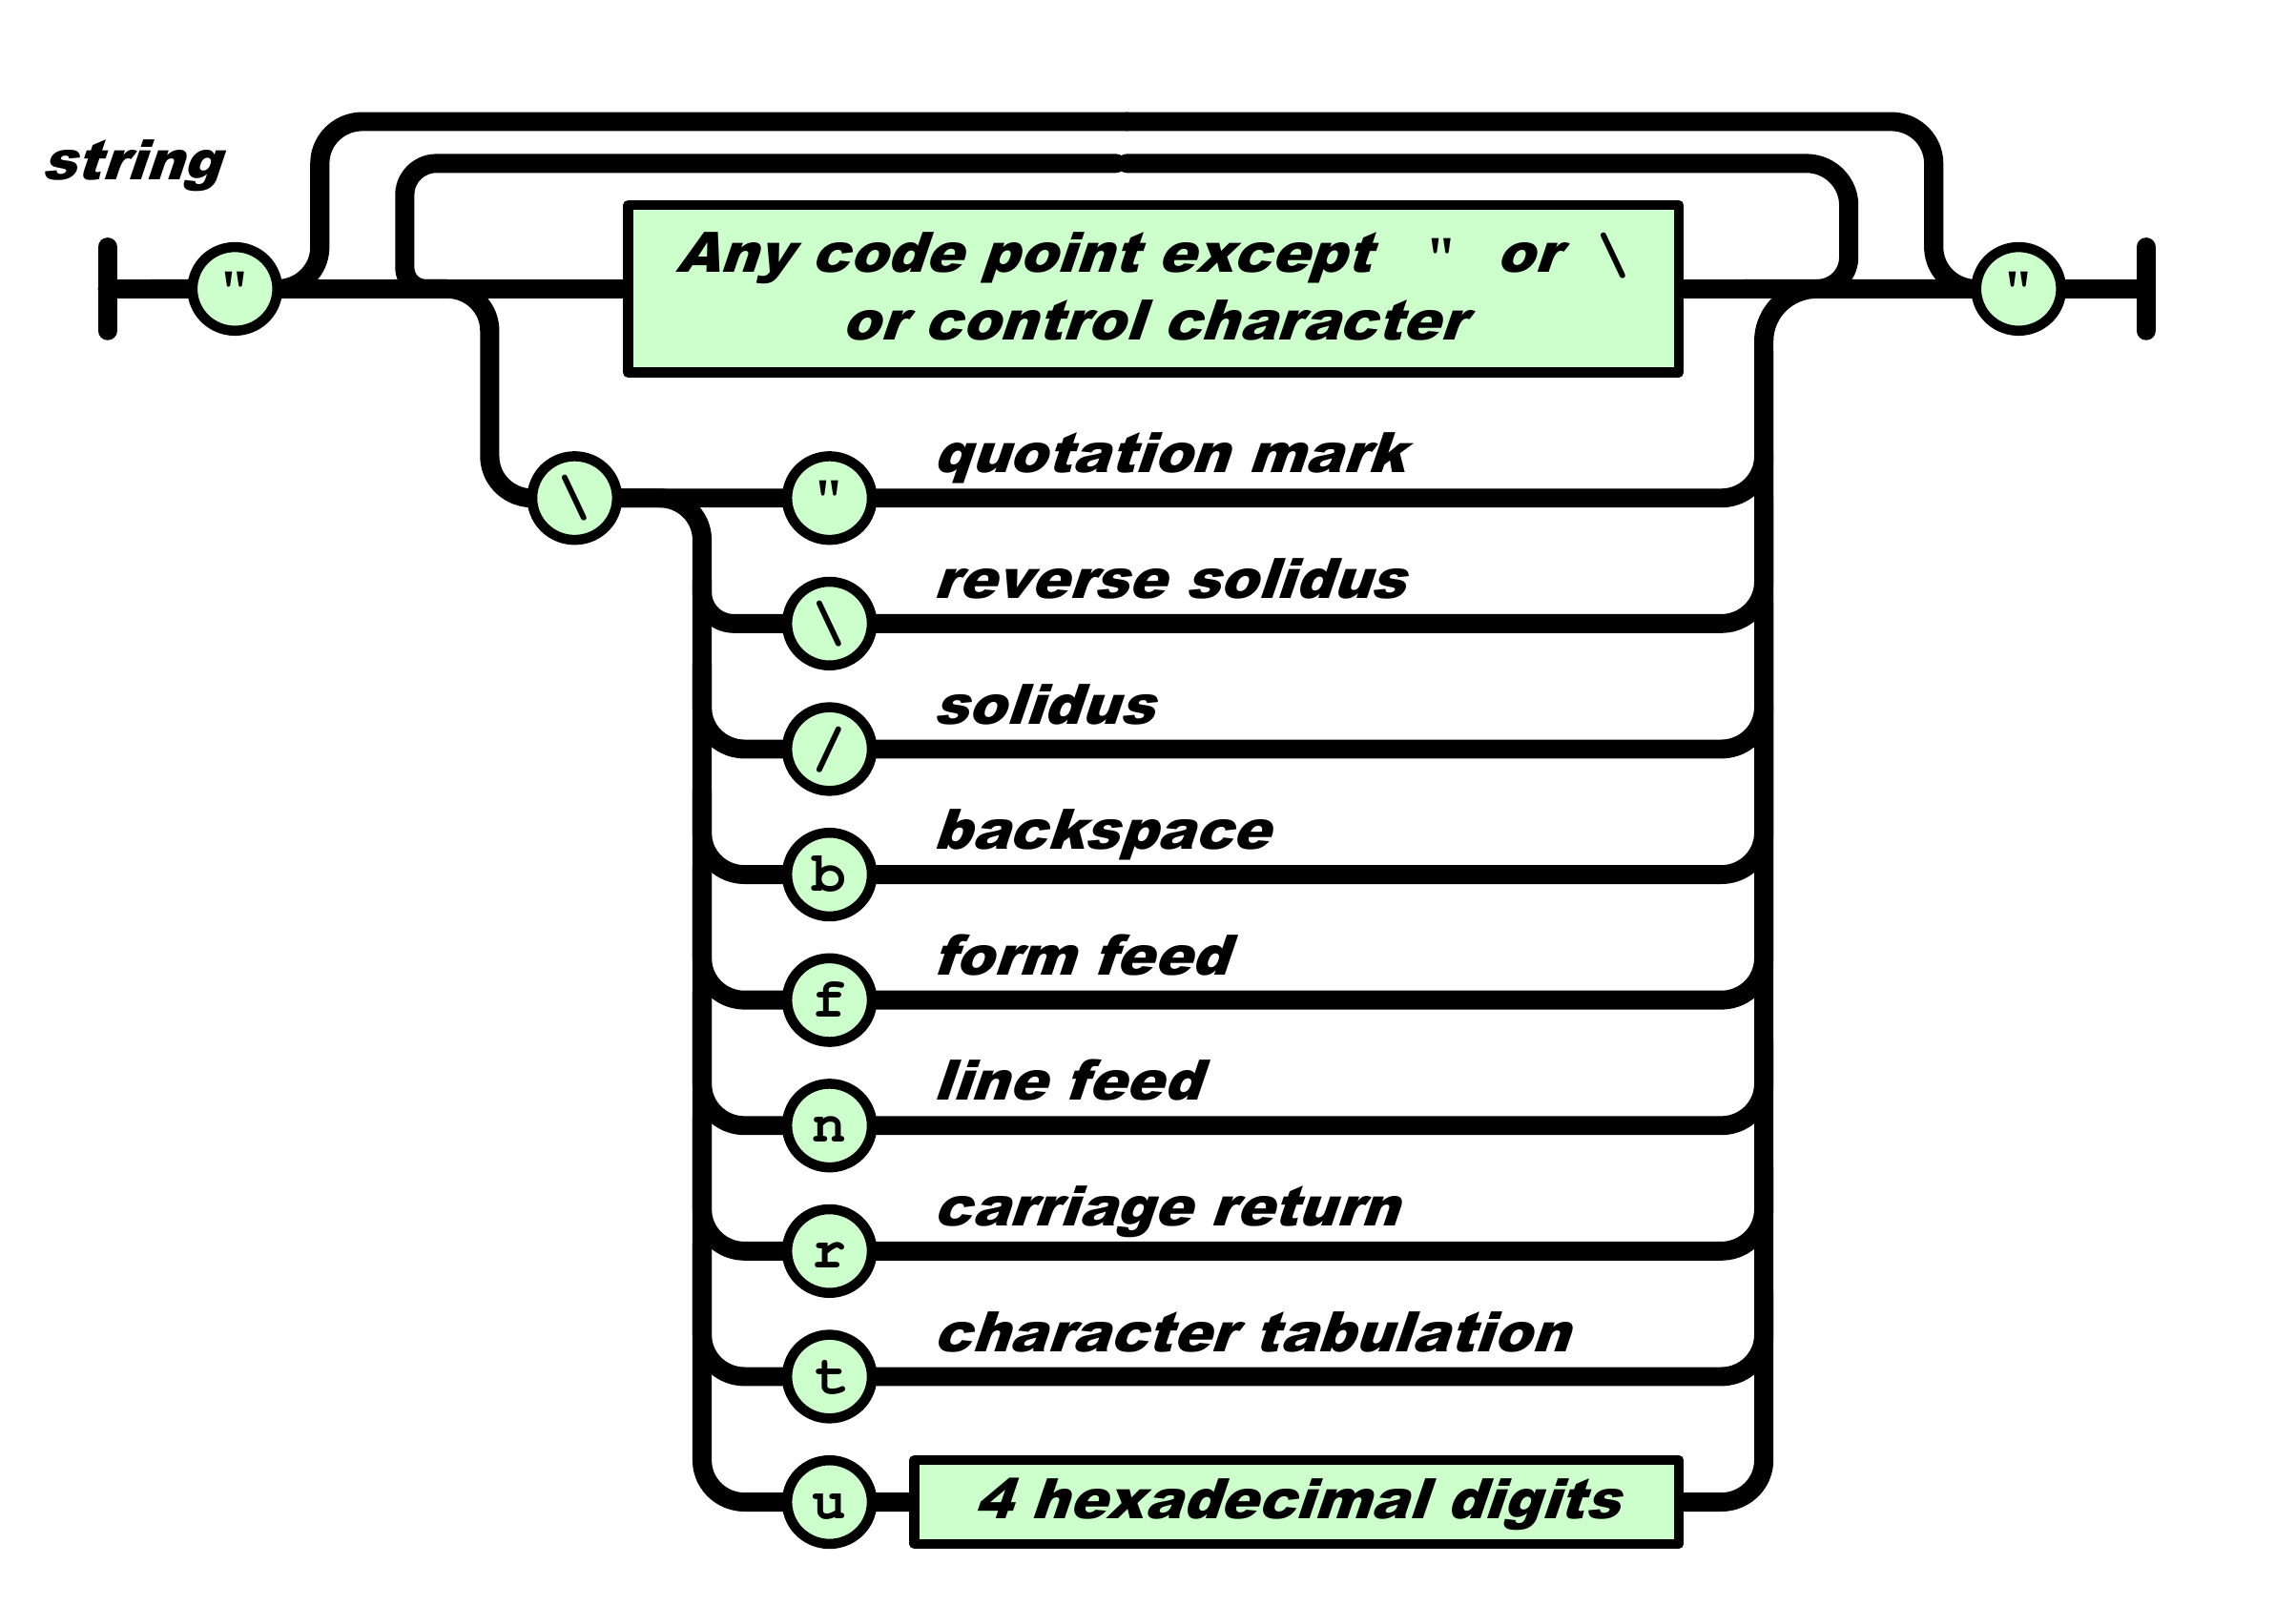
\includegraphics[width=\textwidth]{json_string.png}
				\caption{Niz v JSON\cite{ecma404}}
				\label{fig:json_str}
			\end{figure}
			\begin{figure}[H]
				\centering
				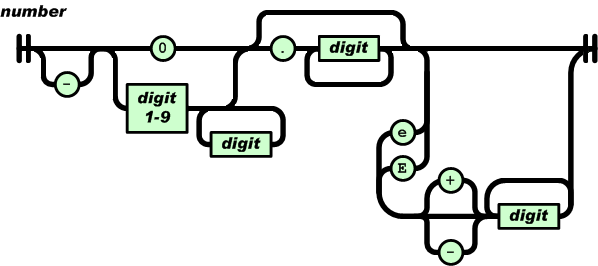
\includegraphics[width=\textwidth]{json_number.png}
				\caption{število v JSON\cite{ecma404}}
				\label{fig:json_num}
			\end{figure}
	\section{Koncepti} % TODO: translate
		\subsection{Abstrakten sistem prepisovanja}
			Abstrakten sistem prepisovanja \angokr{ARS}{abstract rewriting system} je množica objektov $A$ in binarna relacija, ki pove kako preoblikovati te objekte.
			To binarno relacijo imenujemo \textquote{prepisovalna relacija} \cite[chapter, p.~7]{terese} in jo dobimo iz množice pravil.
			ARS se uporabljajo na več področjih, npr. v matematiki, računalništvu, logiki in jezikoslovju.
		\subsection{Sistem prepisovanja členov}
			Sistem prepisovanja členov \angokr{TRS}{term rewriting system} je ARS, ki ima za elemente člene matematičnega izraza.
		\subsection{Sistem prepisovanja nizov}
			Sistem prepisovanja nizov \angokr{SRS}{string rewriting system} ali semi-Thue sistem je ARS, ki ima za elemente nize ali podnize.
		\subsection{Abstraktno sintaktično drevo}
			Aplikacija iz vnosa zgradi abstraktno sintaktično drevo \angokr{AST}{abstract syntax tree}.
			Ko je AST zgrajen, omogoča implementacijo TRS za poenostavljanje izrazov in SRS za pretvarjanje izraza v sintakso jezika \LaTeX{}.
\chapter{Funkcionalnost}
\label{features}
	\section{Glavno okno}
	\label{mainwindow}
		\parbox{\textwidth}{
		Na glavnem oknu je več zavihkov ---
		\textquote{Kalkulator}, \textquote{Napredno}, \textquote{Grafično}, \textquote{Spremenljivke}, \textquote{Konstante} in \textquote{Zgodovina}
		--- vsak s svojo funkcijo.
		\begin{figure}[H]
			\centering
			
\includegraphics{mw_tabs.png}
			\caption{Zavihki na glavnem oknu}
			\label{fig:mw_tabs}
		\end{figure}.}
		\parbox{\textwidth}{
		V zgornjem meniju najdemo nekaj orodji, kot npr. \textquote{Nastavitve} ali \textquote{O programu}
		\begin{figure}[H]
			\centering
			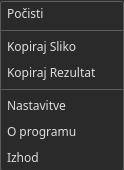
\includegraphics{tools.png}
			\caption{Orodja v zgornjem meniju}
			\label{fig:tools}
		\end{figure}}
		\parbox{\textwidth}{
		Na dnu je pa tudi viden status aplikacije, ki sporoča uporabniku, kaj aplikacija trenutno dela.
		\begin{figure}[H]
			\centering
			
\includegraphics{mw_status.png}
			\caption{Trenutni status aplikacije}
			\label{fig:mw_status}
		\end{figure}}
		\parbox{\textwidth}{
		\subsection{Kalkulator}
			Prvi zavihek je \textquote{preprost} kalkulator.
			Zgoraj je vrstica za vnos računa, pod njo so pa trije gumbi, dva za kopiranje rezultata in en za začetek računanja.
			Računati začne tudi ob pritisku tipke \textquote{Enter}.
			\begin{figure}[H]
				\centering
				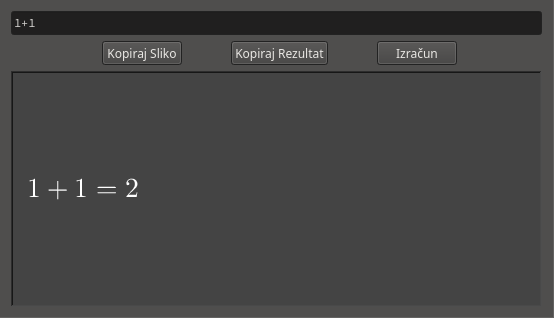
\includegraphics{mw_calc.png}
				\caption{Preprost kalkulator}
				\label{fig:mw_calc}
			\end{figure}}
		\parbox{\textwidth}{
		\subsection{Napredno}
			Napredni kalkulator je razširitev preprostega kalkulatorja.
			Vnosno polje za račun dovoljuje vnašanje večih vrstic, kar pomeni, da je možno uporabiti tudi kompleksnejše strukture kot so zanke ter pogojni stavki.
			Poleg rezultata se pa tudi izriše poenostavljen izraz.
			\begin{figure}[H]
				\centering
				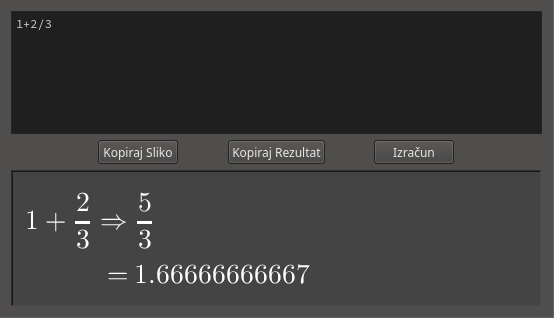
\includegraphics{mw_adv.png}
				\caption{Napredni kalkulator}
				\label{fig:mw_adv}
			\end{figure}}
		\parbox{\textwidth}{
		\subsection{Grafično}
			Vnosno polje je podobno kot v naprednem kalkulatorju, manjka pa gumb \textquote{Kopiraj rezultat}, saj aplikacija v tem načinu nič ne računa, ampak riše grafe funkcij, ki jih pišemo v vnosno polje.
			\begin{figure}[H]
				\centering
				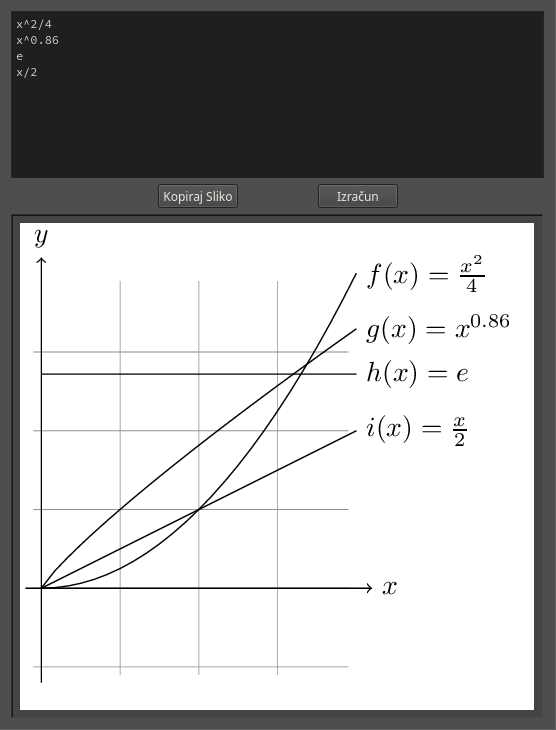
\includegraphics[height=550px]{mw_plot.png}
				\caption{Grafični kalkulator}
				\label{fig:mw_plot}
			\end{figure}}
		\parbox{\textwidth}{
		\subsection{Spremenljivke in Konstante}
			Ta dva zavihka v tabeli prikazujeta vse spremenljivke in konstante, ki so vnesene v programu.
			\begin{figure}[H]
				\centering
				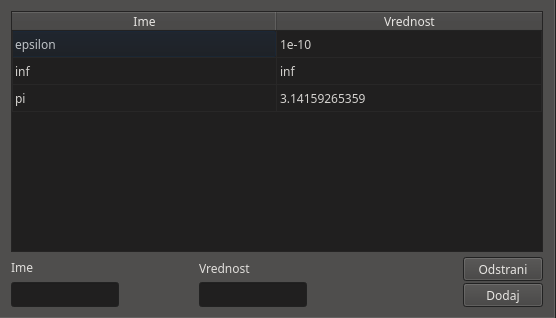
\includegraphics[height=230px]{mw_const.png}
				\caption{Konstante}
				\label{fig:mw_const}
			\end{figure}}
		\parbox{\textwidth}{
			\subsection{Zgodovina}
			Aplikacija beleži zgodovino vnesenih računov.
			\begin{figure}[H]
				\centering
				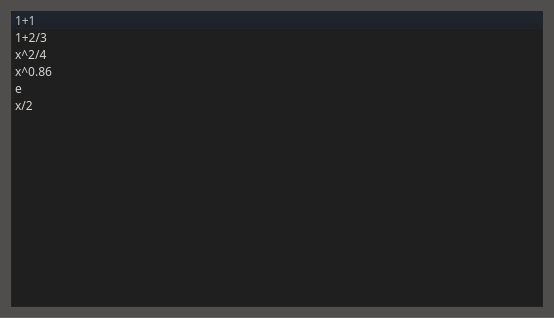
\includegraphics[height=230px]{mw_hist.png}
				\caption{Zgodovina}
				\label{fig:mw_hist}
			\end{figure}}
	\parbox{\textwidth}{
	\section{Nastavitve}
		V nastavitvah lahko nastavljamo jezik, čas prikaza statusa, velikost izrisane slike in barvo slike, lahko pa tudi vklopimo in izklopimo razne funkcije.
		\begin{figure}[H]
			\centering
			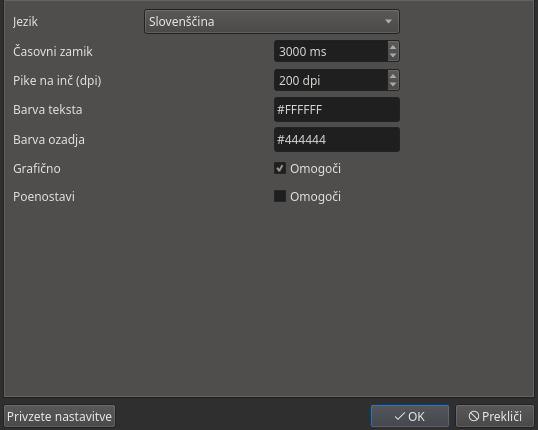
\includegraphics{settings.png}
			\caption{Zgodovina}
			\label{fig:settings}
		\end{figure}
		Na dnu okna najdemo gumba \textquote{OK} in \textquote{Prekliči} ter gumb za nastavitev privzetih vrednosti.}
	\section{Simboli}
	\label{symbol}
		%Aplikacija podpira simbolično računanje s pomočjo AST. % TODO: insert exprtree img
		Aplikacija iz podanega izraza zgradi AST, kar pa reši dva od problemov naloge.
			\subsection{Poenostavljanje izrazov}
				Poenostavljanje izrazov poteka v treh delih:
				\begin{itemize}
					\item ponovno poenostavljanje po preprostih pravilih.
					\item pretvorbe vseh elementov drevesa v ulomke in
					\item ponovno poenostavljanje po preprostih pravilih.
				\end{itemize}
				Prvi del poenostavi izraze kot so $ x + 0 $ in $ x^1 $, drugi del pretvori izraze kot so $ \frac{a}{b} + \frac{c}{d} $ v $ \frac{ad + bc}{bd} $ ali $ 1 + \frac{2}{3} $ v $ \frac{5}{3} $, tretji del pa poenostavi izraze oblike $ \frac{x}{1} $
			\subsection{Pretvorba v \LaTeX{}}
				Za pretvorbo v \LaTeX{} se program preprosto spusti po drevesu in na primer za ulomke izpiše \texttt{\{$\backslash$frac\{števec\}\{imenovalec\}\}}. Z le par preprostimi pravili dokaj zanesljivo prepiše cel izraz.
				
\chapter{Implementacija}
\label{impl}
	\section{Glavno okno}
	\label{mainwindow_impl}
		\subsection{Inicializacija}
		\label{constructor}
			Aplikacija najprej naloži nastavitve in postavi par spremenljivk na začetne vrednosti, nato pa začne klicati podprograme za inicializacijo posameznih logičnih enot. % TODO: rewrite
			Potem poveže signal, ki se sproži, ko je rezultat obdelan, na režo, ki rezultat posreduje izrisovalcu.
			Na koncu še vpiše ves tekst v aplikacijo.
			
			\subsubsection{KLFBackend}
				Podprogram najde nastavitve \LaTeX{} ozadja in z njimi naredi nov \codequote{KLFPreviewBuilderThread}. % TODO: retranslate backend
			
			\subsubsection{Exprtk}
				Podprogram naredi nov \codequote{MufExprtkBackend} in poveže signal za konec računanja in signal za napake na njihove reže.
			
			\subsubsection{Glavno okno}
				Podprogram najprej kliče podprogram za inicializacijo gornjega menija in poskrbi, da ko se spremeni jezik v knjižnici za prevajanje, se tudi posodobi tekst.
			
			\subsubsection{Meni}
				Podprogram naredi nov \codequote{MufMenu} in poveže elemente menija na reže, ki bojo izvedle želeno akcijo.
			
			\subsubsection{Spremenljivke in konstante}
				Podprogram naredi nove \codequote{MufSymbolListView\_w}-je, jih doda v njihove zavihke, jih posodobi s podatki iz \codequote{Exprtk}-ja in poveže gumbe za dodajanje in odstranjevanje spremenljivk in konstant.
			
			\subsubsection{Funkcije}
				Podprogram najde pot do definicij funkcij in s to potjo naredi nov \codequote{MufFunctions}.
			
			\subsubsection{Kalkulator}
				Vsi trije podprogrami za inicializacijo zavihkov s kalkulatorji povežejo signale, ki sprožijo računanje na reže, ki začnejo računanje in povežejo gumbe za kopiranje rezultata.
				Nato nastavijo še kazalec na vnosno polje.
			
			\subsubsection{Nastavitve}
				Podprogram naredi nov \codequote{MufSettings\_w}.
				Nato najde pot do jezikovnih datotek in jezike doda v spisek jezikov.
			
			\subsubsection{Posodobitev teksta}
				Podprogram v program vpiše na novo prevedene ključe in pokliče podprograme štirih drugih objektov: spremenljivke, konstante, nastavitve in gornji meni, ki pa naredijo podobno.
		
		\subsection{Potek računanja}
		\label{calculate}
			Za računanje so zadolžene tri skupine funkcij, vsaka za svoj način računanja.
			Vsaka skupina funkcij je označena s svojo končnico, -\texttt{\textbraceleft$\emptyset$\textbraceright} za navadni način, --\texttt{\emph{\_adv}} za napredni način in --\texttt{\emph{\_plot}} za grafični način. % TODO: suffix
			Ker so si te trije načini računanja zelo podobni, se je veliko kode ponavljalo, kar lahko povzroča napake.
			To sem rešil tako, da sem združil podobne funkcije v eno, pustil sem pa nekaj ključnih funkcij, ki skrbijo za celoten potek izračuna.\odstavek
			Najprej bom opisal celoten potek, potem pa bom še povedal kaj se spremeni v različnih skupinah funkcij.
			Računanje se začne v funkciji \codequote{compute}, ki s pomočjo Qt-ovih funkcij \codequote{connect} in \codequote{disconnect} nadzira, katera skupina funkcij naj se uporablja, kliče pa tudi funkciji \codequote{updateHistory} in \codequote{updateExprtkInput}, ki posodobita zgodovino in račun v knjižnici \textquote{Exprtk}.
			Ko \textquote{Exprtk} obdela račun in vrne rezultat, je ta posredovan funkciji, ki poskusi odpraviti napake, ki nastanejo zaradi omejitev jezika.
			Ko je rezultat obdelan se začne izvajati funkcija \codequote{updatePreviewBuilderThreadInput}, ki nastavi nastavitve KLF-ja, pretvori izraz v \LaTeX{} in začne risanje.
			Ko \textquote{KLFBackend} izriše izraz, se slika pošlje funkciji, ki to sliko postavi v aplikacijo.
			\odstavek
			Med funkcijami iz različnih skupin ni veliko razlik, spremenijo se le imena spremenljivk, kar je težko spreminjati, glede na trenuten potek izvajanja programa, lahko pa vidimo bistvene razlike v funkciji \codequote{updatePreviewBuilderThreadInput}.\\
			\parbox{\textwidth}{
			\subsubsection{Navadni način}
				V navadnem načinu funkcija nastavi \textquote{KLFBackend} nastavitve:
				\begin{alignitemize}
					\codequote{input.preamble} &nastavi na \codequote{$\backslash$usepackage\{amssymb,mathtools,mathrsfs\}}\\
					\codequote{input.mathmode} &nastavi na \codequote{$\backslash$[ ...\:$\backslash$]}\\
					\codequote{input.bypasstemplate} &nastavi na \codequote{false}\\
					\codequote{input.latex} &nastavi na \codequote{vhod = vrednost}
				\end{alignitemize}
			}
			\parbox{\textwidth}{
			\subsubsection{Napredni način}
				V naprednem načinu funkcija nastavi \textquote{KLFBackend} nastavitve:
				\begin{alignitemize}
					\codequote{input.preamble} &ne nastavi\\
					\codequote{input.mathmode} &ne nastavi\\
					\codequote{input.bypasstemplate} &nastavi na \codequote{true}\\
					\codequote{input.latex} &nastavi na:
				\end{alignitemize}
				\begin{figure}[H]
					\centering
					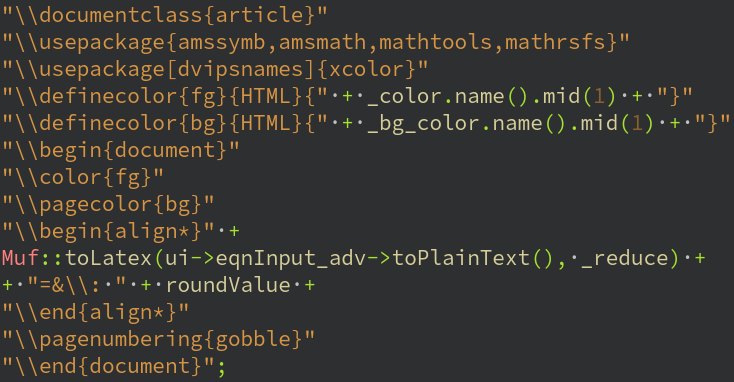
\includegraphics[width=\textwidth]{latex_adv.png}
					\caption{input.latex}
					\label{fig:latex_adv}
				\end{figure}}
			\parbox{\textwidth}{
			\subsubsection{Grafični način}
				V grafičnem načinu funkcija nastavi \textquote{KLFBackend} nastavitve:
				\begin{alignitemize}
					\codequote{input.preamble} &ne nastavi\\
					\codequote{input.mathmode} &ne nastavi\\
					\codequote{input.bypasstemplate} &nastavi na \codequote{true}\\
					\codequote{input.latex} &nastavi tako:
				\end{alignitemize}
				\begin{figure}[H]
					\centering
					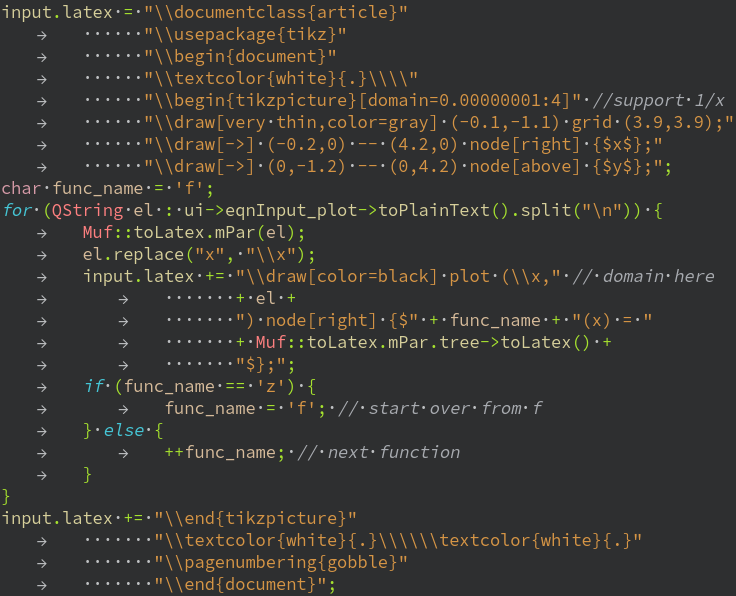
\includegraphics[width=\textwidth]{latex_plot.png}
					\caption{input.latex}
					\label{fig:latex_plot}
				\end{figure}}
\chapter{Navodila za uporabo}
	\section{Jezik kalkulatorja}
		\begin{alignitemize}
			Osnovni operatorji: &\texttt{+, -, *, /, \%, \^{}} \\
			Prireditev: &\texttt{:=, +=, -=, *=, /=, \%=}\\
			Enakosti in neenakosti: &\texttt{=, ==, <>, !=, <, <=, >, >=}\\
			Logični operatorji: &\group{225pt}{and, mand, mor, nand, nor, not, or, shl, shr, xnor, xor, true, false}\\
			Funkcije: &\group{375pt}{abs, avg, ceil, clamp, equal, erf, erfc, exp, expm1, floor, frac, log, log10, log1p, log2, logn, max, min, mul,  ncdf, nequal, root, round, roundn, sgn, sqrt, sum, swap, trunc}\\
			Trigonometrija: &\group{330pt}{acos, acosh, asin, asinh, atan, atanh, atan2, cos, cosh, cot, csc, sec, sin, sinc, sinh, tan, tanh, hypot, rad2deg, deg2grad, deg2rad, grad2deg}\\
			Nadzor pretoka: &\group{250pt}{if-then-else, trojiški pogojni operator (?:), switch-case, return}\\
			Zanke: &\texttt{while, for, repeat-until, break, continue}
		\end{alignitemize}
		Različni stavki so ločeni s podpičjem (;), kalkulator bo pa izpisal vrednost zadnjega izraza.
		\odstavek
		Aplikacija podpira tudi definicijo funkcij, ki se naložijo ob zagonu programa.
		Definicije funkcij se nahajajo v mapi \textquote{function}.
		V tej mapi so funkcije razdeljene na \textquote{skupine} predstavljene s podmapami.
		Na primer funkcija \codequote{add} se nahaja v datoteki \textquote{math} v mapi \textquote{stl}, torej lahko rečemo da pripada knjižnici \textquote{math} iz skupine \textquote{stl}.
		Imena funkcij se ne smejo ponavljati.
		\odstavek
		Aplikacija v večini primerov spremenljivke obravnava kot globalne spremenljivke. Uporabnik jih preprosto inicializira \codequote{x := 3} in potem jih lahko prosto uporablja.
		Na voljo so pa tudi lokalne spremenljivke, ki se uporabljajo, ko v izrazu ni nobenih zunanjih (globalnih) spremenljivk, vendar so vse uporabljene spremenljivke definirane v izrazu. V tem primeru \emph{moramo} uporabiti rezervirano besedo \codequote{var}. Nekaj primerov preprostih izrazov, ki uporabljajo le lokalne spremenljivke so:
		\begin{itemize}
			\item \texttt{1 + 2}
			\item \texttt{var x := 3; 2 * x - 3}
			\item \texttt{var x := 3; var y := abs(x - 8); x - y / 7}
		\end{itemize}
		Sintaksa kontrolnih struktur je zelo podobna C, C++ ipd.:
		\begin{itemize}
			\item \parbox{\textwidth}{\vspace{5px}\setstretch{0.8}\texttt{if(cond) \{\\\wdot\qquad expr1;\\ \wdot\qquad expr2;\\\};}\vspace{5px}}
			\item \parbox{\textwidth}{\vspace{5px}\setstretch{0.8}\texttt{if(cond) \{\\\wdot\qquad expr1;\\ \wdot\qquad expr2;\\\} else \{\\\wdot\qquad expr3;\\ \wdot\qquad expr4;\\\};}\vspace{5px}}
			\item \parbox{\textwidth}{\vspace{5px}\setstretch{0.8}\texttt{switch \{\\\wdot\qquad case cond: expr1;\\ \wdot\qquad case cond: expr2;\\\};}\vspace{5px}}
			\item \parbox{\textwidth}{\vspace{5px}\setstretch{0.8}\texttt{while(cond) \{\\\wdot\qquad expr1;\\ \wdot\qquad expr2;\\\};}\vspace{5px}}
			\item \parbox{\textwidth}{\vspace{5px}\setstretch{0.8}\texttt{repeat \\\wdot\qquad expr1;\\ \wdot\qquad expr2;\\ untill(cond);}\vspace{5px}}
			\item \parbox{\textwidth}{\vspace{5px}\setstretch{0.8}\texttt{for(init;cond;iter) \{\\\wdot\qquad expr1;\\ \wdot\qquad expr2;\\\};}\vspace{5px}}
			\item \texttt{break} in \texttt{break[]} zapusti zanko in vrne vrednost znotraj \texttt{[]}.
			\item \texttt{continue} spusti iteracijo in nadaljuje z izvajanjem zanke
			\item Trojiški operator: cond ? exprT : exprF
			\item \texttt{~(expr1, expr2) == expr2}:\\
			Izračuna vse pod-izraze potem pa vrne zadnji pod-izraz.
			\item \parbox{\textwidth}{\vspace{5px}\setstretch{0.8}\texttt{[*] \{\\\wdot\qquad case cond: expr1;\\ \wdot\qquad case cond: expr2;\\\};}\vspace{5px}}
			Za razliko od \texttt{switch-case} bo \texttt{[*]} izračunal vse izraze za katere je \texttt{cond} enak \texttt{true}
		\end{itemize}
		\subsection{Vhodno/izhodne operacije}
			Exprtk pozna dve vrsti I/O operacij (vhodno/izhodnih, iz angl. Input/Output):
			\begin{itemize}
				\item Standardne vhodno/izhodne operacije:
				\begin{enumerate}
					\item \texttt{print}
					\item \texttt{println}
				\end{enumerate}
				\item Datotečne vhodno/izhodne operacije:
				\begin{multicols}{3}
				\begin{enumerate}
					\item \texttt{open}
					\item \texttt{close}
					\item \texttt{write}
					\item \texttt{read}
					\item \texttt{getline}
					\item \texttt{eof}
				\end{enumerate}
				\end{multicols}
			\end{itemize}
		\subsection{Vektorske operacije}
			%TODO: basic vectors
			Na voljo so tudi dodatne vektorske funkcije:
			\begin{multicols}{3}
			\begin{enumerate}
				\item \texttt{all\_true}
				\item \texttt{all\_false}
				\item \texttt{any\_true}
				\item \texttt{any\_false}
				\item \texttt{count}
				\item \texttt{copy}
				\item \texttt{rotate-left}
				\item \texttt{rotate-right}
				\item \texttt{shift-left}
				\item \texttt{shift-right}
				\item \texttt{sort}
				\item \texttt{nth\_element}
				\item \texttt{iota}
				\item \texttt{sumk}
				\item \texttt{axpy}
				\item \texttt{axpby}
				\item \texttt{axpyz}
				\item \texttt{axpbyz}
				\item \texttt{axpbyz}
				\item \texttt{dot}
				\item \texttt{dotk}
			\end{enumerate}
			\end{multicols}
			
\chapter{Rezultati in ugotovitve}


%\chapter{Viri in literatura}
%{qt docs}\\
%{tex.stackexchange}\\
%{stackoverflow.net}\\
%{exprtk pages}\\

\newpage
\printbibliography

\end{document}


























































